\documentclass[10pt,a4paper]{article}
\usepackage[margin=24mm]{geometry}
\usepackage[T1]{fontenc}
\usepackage{lmodern,amsmath,amssymb,graphicx,booktabs,microtype,placeins}
\usepackage[colorlinks=true,linkcolor=blue,urlcolor=blue]{hyperref}
\setlength{\emergencystretch}{2em}
\graphicspath{{figures/}}
\newcommand{\dd}{\,\mathrm{d}}
\renewcommand{\thefigure}{S\arabic{figure}}
\renewcommand{\thetable}{S\arabic{table}}
\newcommand{\NominalTable}{%
\begin{table}[htbp]
\centering
\caption{Nominal inputs for the reported calculations.}\label{tab:parameters}
\begin{tabular}{ll}\toprule
Quantity & Value\\\midrule
Substrate radius $R$ & $12.7$ mm\\
Substrate thickness $L$ & $5.0$ mm\\
Beam radius $w_0$ & $3.81$ mm ($0.3R$)\\
Full-plane absorbed power $P_{\rm abs}$ & $0.110$ W\\
Thermal conductivity $k$ & $1.38$ W\,m$^{-1}$\,K$^{-1}$\\
Density $\rho$ & $2203$ kg\,m$^{-3}$\\
Specific heat $c_p$ & $772$ J\,kg$^{-1}$\,K$^{-1}$\\
Ambient temperature $T_\infty$ & $300$ K\\
Convection coefficient $h_{\rm conv}$ & $10$ W\,m$^{-2}$\,K$^{-1}$\\
Emissivity $\epsilon$ & $0.85$\\
Linearized total loss $h_{\rm eff}$ & $15.2054$ W\,m$^{-2}$\,K$^{-1}$\\
Thermo-optic coefficient $\gamma_T$ & $9.6\times10^{-6}$ K$^{-1}$\\
Reference wavelength; refractive indices & $1064$ nm; $n_i=1$, $n_s=1.44963$\\
Entrance-pupil radius $a$ & $0.9R$\\\bottomrule
\end{tabular}
\par\smallskip\begin{minipage}{.96\linewidth}\footnotesize $\gamma_T$ is a retained nominal value tabulated at $643.8$ nm, not a wavelength-specific measurement at $1064$ nm. The intercepted disk power is obtained by integrating the prescribed flux on the finite face.\end{minipage}
\end{table}}

\newcommand{\SteadyFieldTable}{%
\begin{table}[htbp]
\centering
\caption{Steady temperature rises and sampled OPD-PV.}\label{tab:steadyfields}
\begin{tabular}{lrrrr}\toprule
$\theta$ & Front center (K) & Midplane center (K) & Rear center (K) & OPD-PV (nm)\\\midrule
$0^\circ$ & 11.921 & 7.656 & 6.716 & 166.503\\
$30^\circ$ & 11.336 & 7.537 & 6.656 & 168.771\\
$60^\circ$ & 9.303 & 6.959 & 6.314 & 154.105\\\bottomrule
\end{tabular}
\par\smallskip\begin{minipage}{.96\linewidth}\footnotesize OPD-PV uses the saved $201\times201$ physical transmitted-pupil grid. Continuous numerical extrema are reported separately in Supplement 1; FEM comparisons use their own discrete common domain.\end{minipage}
\end{table}}

\newcommand{\TransientRefinementTable}{%
\begin{table}[htbp]
\centering
\caption{Largest transient FEM refinement changes across temperature and OPD metrics (percent).}\label{tab:refinement}
\begin{tabular}{lrrrr}\toprule
$\theta$ & Transverse & Axial & Time & Joint\\\midrule
$0^\circ$ & 0.104616 & 0.029993 & 0.025763 & 0.125259\\
$30^\circ$ & 0.099671 & 0.029973 & 0.025837 & 0.118577\\
$60^\circ$ & 0.088451 & 0.029925 & 0.026017 & 0.105834\\
Target & $0.5$ & $0.5$ & $0.1$ & $0.5$\\\bottomrule
\end{tabular}
\par\smallskip\begin{minipage}{.96\linewidth}\footnotesize Maxima include the positive observation times from $0.0025$ to $75$ s. The $0.001$ s frame is recorded separately as a diagnostic; the exact zero initial condition and all-step physical checks remain independent requirements.\end{minipage}
\end{table}}

\newcommand{\ValidationTable}{%
\begin{table}[htbp]
\centering
\caption{Optical differences between FEM and the semi-analytical calculation (percent).}\label{tab:comparison}
\begin{tabular}{lrrr}\toprule
$\theta$ & Steady $E_V$ & Transient $E_V$ & Transient $E_{W,\infty}$\\\midrule
$0^\circ$ & 0.004220 & 0.071263 & 0.090254\\
$30^\circ$ & 0.000523 & 0.054394 & 0.085118\\
$60^\circ$ & 0.005440 & 0.046821 & 0.082570\\\bottomrule
\end{tabular}
\par\smallskip\begin{minipage}{.96\linewidth}\footnotesize Steady values use the finest FEM mesh. Transient values are maxima over sampled times from $2.5$ ms to $75$ s and use the FEM candidate examined by the separate refinements. All denominators are the semi-analytical PV on the common pupil. Supplement 1 retains full temperature and optical statistics, including $1$ ms diagnostics.\end{minipage}
\end{table}}

\title{Supplement 1: Numerical details for the Fourier--Bessel model of obliquely heated cylindrical optics}
\author{Zhongwei Yang, Jing Wen, Wei Li, Tingrui Li, Bohui Chen, and Liang Yang}
\date{27 October 2026}
\begin{document}
\maketitle
\section{Modal references and observation times}
The steady temperature reference uses $M=14$, $N=32$, a $2400\times256$ source grid, and 64 ray points; the enlarged temperature reference uses $M=16$, $N=40$, a $3200\times512$ source grid, and 80 ray points.
The transient temperature references use the same two transverse configurations with $J=512$ and $768$, respectively.
The selected steady configuration is $M=6$, $N=8$, $400\times32$, and 16 ray points; the selected transient configuration is $M=10$, $N=20$, $J=256$, $1200\times128$, and 32 ray points.
The finite-reference target is $0.1\%$, with additional transient temperature-gradient and near-surface depth checks.
For optical evaluation, the steady reference uses $M=10$, $N=20$, $1200\times128$, and 32 ray points.
The transient optical reference uses $M=14$, $N=28$, $J=384$, $1800\times256$, and 64 ray points; a separate check doubles the selected transient ray quadrature from 32 to 64 points.
All optical evaluations use the matched $1064$ nm, $300$ K inputs in the main-text parameter table.

The positive observation times are $0.001$, $0.0025$, $0.01$, $0.05$, $0.1$, $0.625$, $2.5$, $20$, $50$, and $75$ s.
The zero initial field and the separate long-time evaluation are checked independently.
The $1$ ms frame belongs to the modal-resolution comparisons and is retained as a diagnostic outside the FEM refinement criteria.
Those FEM criteria apply at the sampled times from $2.5$ ms to $75$ s.
The one-parameter steady sweeps in Fig.~\ref{fig:supp-resolution} complement these joint modal-reference checks.
The entrance-pupil grids in this diagnostic are not nested, so sampled extrema need not vary monotonically.

% Source: outputs/convergence_diagnostic/20261017T093231672765Z_4809a8b0_modal_sum_continuation_sweeps_a1/summary.json
\begin{figure}[!htbp]
\centering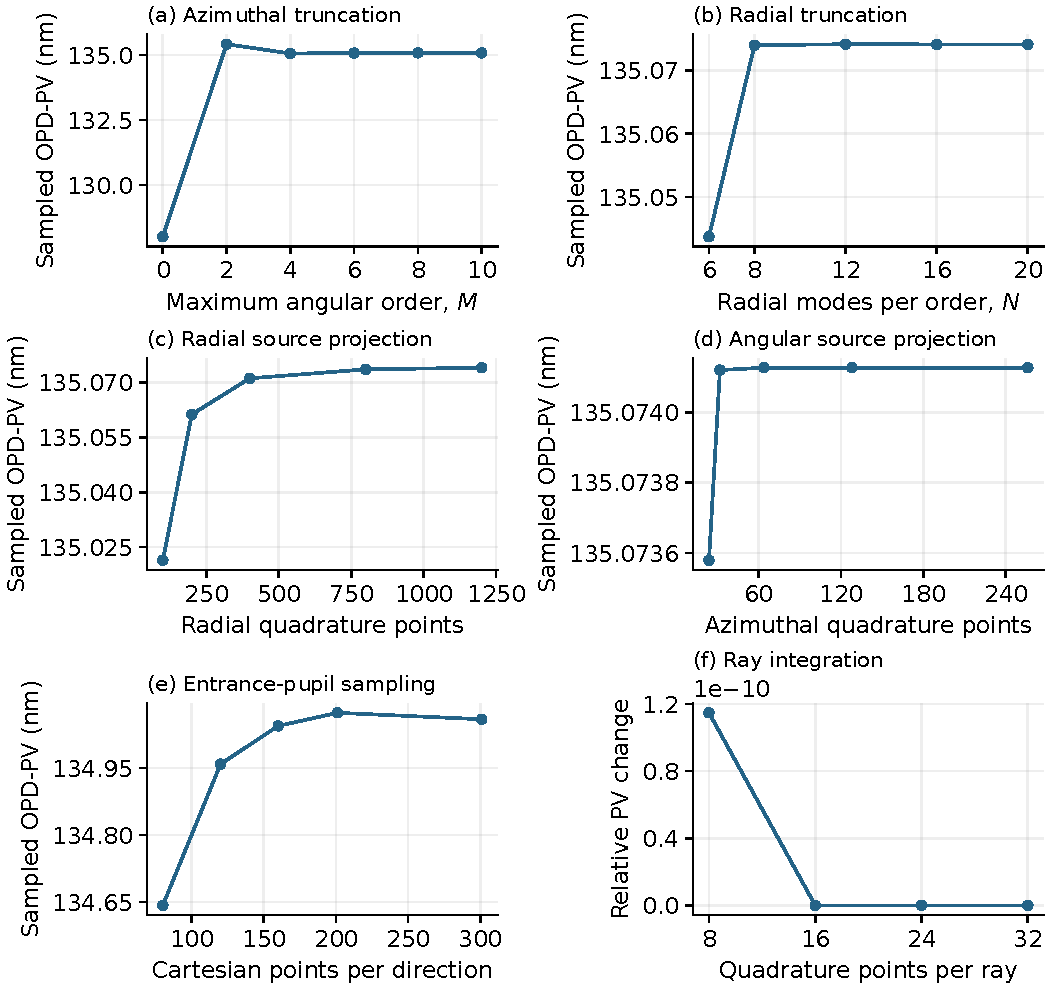
\includegraphics[width=\linewidth]{supp_steady_resolution.pdf}
\caption{One-parameter steady resolution sweeps at $60^\circ$.
Panels (a)--(e) show sampled physical-pupil OPD-PV as a function of each numerical setting.
Panel (f) shows the relative PV change with respect to the finest ray quadrature in that sweep; its final zero is the reference by definition.
Unless varied, the settings are $M=10$, $N=20$, $1200\times256$ source-projection points, a $201\times201$ entrance-pupil grid, and $32$ ray points.
These diagnostic settings differ from the selected steady configuration; the curves complement the modal-reference checks rather than giving errors against an exact solution.}
\label{fig:supp-resolution}
\end{figure}
\FloatBarrier

\section{Finite-element discretization}
The steady FEM uses $2113$ or $8321$ transverse degrees of freedom and $32$ or $64$ uniform quadratic axial elements.
The candidate, transverse, axial, and joint configurations therefore contain $137345$, $540865$, $272577$, and $1073409$ total degrees of freedom.
For the transient FEM, the transverse counts are unchanged.
Two-face axial grading uses $88$ elements ($177$ axial degrees of freedom) for the candidate and $174$ elements ($349$ axial degrees of freedom) for the axial reference.
The candidate and joint transient configurations contain $374001$ and $2904029$ total degrees of freedom.

The ten observation intervals use $128$ time steps each, except $0.1$--$0.625$ s, which uses $1024$, for $2176$ steps overall.
Time and joint references halve the step in every interval.
A backward-Euler step starts the calculation and restarts BDF2 when the step ratio exceeds $1.5$.
The transient calculation uses a consistent mass matrix.
Initial conditions, energy balance, weak-equation residuals, Robin-loss diagnostics, and applied-load quadrature are assessed separately from mesh and time-step refinement.

Figure~\ref{fig:supp-fem-refinement} shows the temperature-refinement changes at each positive observation time.

% Source: outputs/fem_convergence_validation/20261017T032513109092Z_ce9843f7_defect_continuation_transient_fem_convergence_a1/verification.json
\begin{figure}[!htbp]
\centering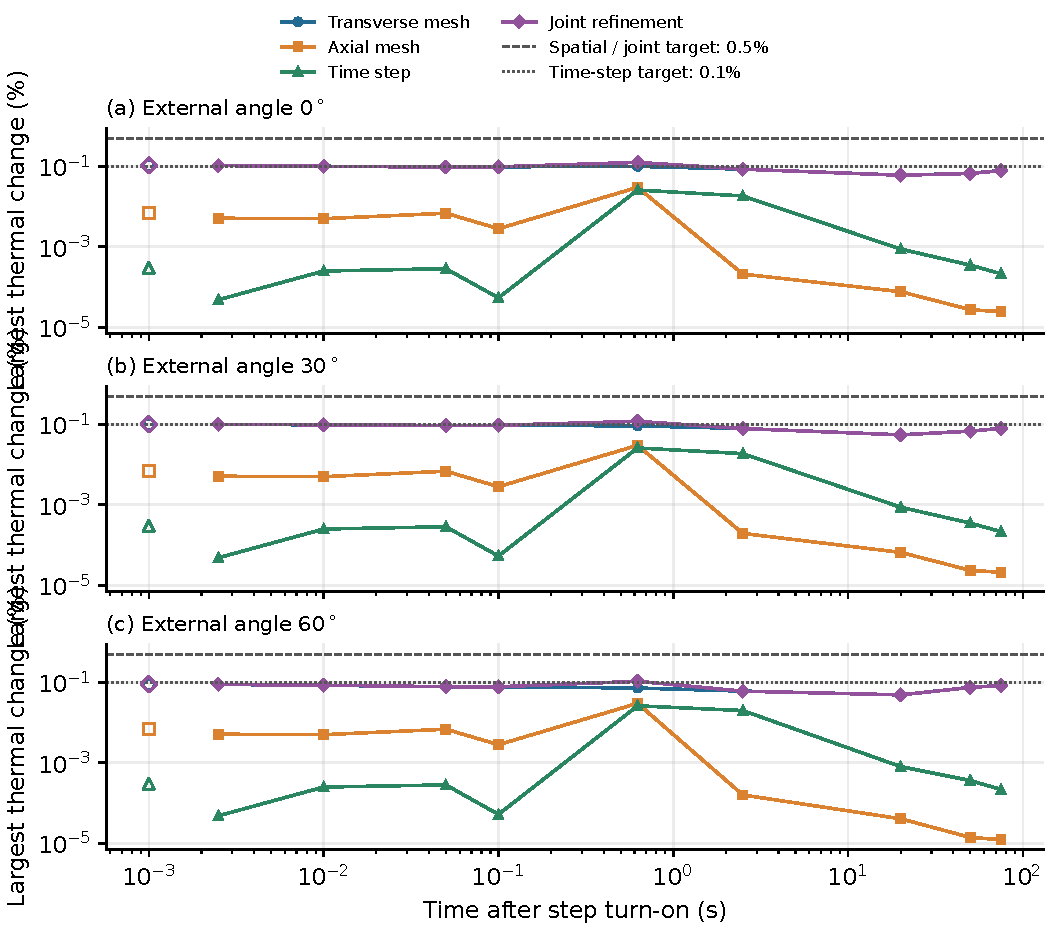
\includegraphics[width=.91\linewidth]{supp_transient_fem_refinement.pdf}
\caption{Transient FEM temperature-refinement changes for (a) $0^\circ$, (b) $30^\circ$, and (c) $60^\circ$.
Each curve compares the candidate FEM with the indicated refined FEM and takes the maximum across the recorded temperature metrics at a given time.
Filled markers and their connecting lines show the sampled refinement interval; unconnected open markers show the $1$ ms diagnostic.
Temperature norms cover the three fixed planes and seven diffusion-depth samples; they use the largest corresponding refined-reference norm across these depths before $0.625$ s and a separate norm at each depth thereafter.
Horizontal lines mark the spatial/joint and temporal refinement targets.
These curves assess the thermal FEM discretization; optical method-to-method differences on the refracted paths are reported separately in Table~\ref{tab:supp-comparison}.}
\label{fig:supp-fem-refinement}
\end{figure}
\FloatBarrier

\begin{samepage}
The Gaussian front-face load uses quadrature order 10 and is checked against order 14, with changes satisfying the $10^{-5}$ relative target.
FEM ray integrals are divided at crossed element boundaries and use three-point Gauss quadrature on every segment.
The tensor-product quadratic field is quartic along a straight segment, so this quadrature is exact for the represented field up to arithmetic error.

\end{samepage}

\section{Sampling and comparison conventions}
The thermal FEM refinement comparisons use a $201\times201$ Cartesian thermal grid on the common mesh domain.
The optical mask requires both physical rear-face transmission and inclusion in the common FEM polygon.
The transient cross-method temperature comparisons use a polar Gauss-radius/uniform-azimuth sampling with $201\times201$ points; optical comparisons use a $101\times101$ Cartesian entrance grid.
Cross-method field differences are evaluated on the common samples.

For the cross-method comparisons, weighted temperature $L^2$ differences are divided by the reference $L^2$ norm, and maximum differences are divided by the reference maximum magnitude.
At $t\geq0.625$ s, each section supplies its own denominator.
At earlier positive times, each norm uses the largest reference value across the three sections, avoiding a denominator set by an almost unheated rear plane.
OPD is de-pistoned on the common pupil before field differences are formed.
Both the optical field differences and the PV differences use the semi-analytical PV as their denominator.

The steady scalar results in the main-text table use the saved $201\times201$ physical-pupil samples.
Continuous numerical extrema are a separate multistart SLSQP estimate on the transmitted pupil.
For $0^\circ$, $30^\circ$, and $60^\circ$, the saved continuous steady PV values are $145.958$, $147.973$, and $135.075$ nm, respectively.
They are distinct from both the main-text sampled PV values and the discrete common-domain FEM-comparison PV values.
For the transient fields, continuous-pupil OPD-PV estimates at $0.625$ s are $13.080$, $12.212$, and $8.502$ nm for $0^\circ$, $30^\circ$, and $60^\circ$; at $75$ s they are $137.055$, $137.592$, and $123.391$ nm.
The main-text transient values instead use the saved physical-pupil samples, consistently with its steady and thermal-order comparisons.

\section{Full recorded comparison range}
The following table retains all positive comparison times, including the $1$ ms diagnostic.
The main-text table restricts the transient maxima to the sampled $2.5$ ms--$75$ s FEM-refinement range.
The steady entries are unchanged between the two summaries.
These are method-to-method differences at the recorded numerical resolutions.
\begin{table}[htbp]
\centering
\caption{Differences between FEM and the semianalytical solution (percent).}\label{tab:supp-comparison}
\begin{tabular}{llrrr}\toprule
Case & $\theta$ & Temperature $L^\infty$ & OPD $L^\infty$/PV & OPD-PV\\\midrule
Steady & $0^\circ$ & 0.031420 & 0.005848 & 0.004220\\
Steady & $30^\circ$ & 0.023794 & 0.004131 & 0.000523\\
Steady & $60^\circ$ & 0.111849 & 0.071196 & 0.005436\\
Transient & $0^\circ$ & 0.136599 & 0.092695 & 0.071263\\
Transient & $30^\circ$ & 0.128643 & 0.094190 & 0.054396\\
Transient & $60^\circ$ & 0.119119 & 0.095791 & 0.046819\\\bottomrule
\end{tabular}
\par\smallskip\begin{minipage}{.96\linewidth}\footnotesize Steady rows use the finest FEM solution; transient rows use the FEM candidate and maximize over all positive comparison times, including $1$ ms. The semianalytical solution supplies the reference denominators. These differences are reported without imposing a separate cross-method pass threshold.\end{minipage}
\end{table}

\clearpage
\section{Steady spatial comparison}
The steady $60^\circ$ comparison shows the independent nodal and modal representations on their common domain.
\begin{figure}[!htbp]
\centering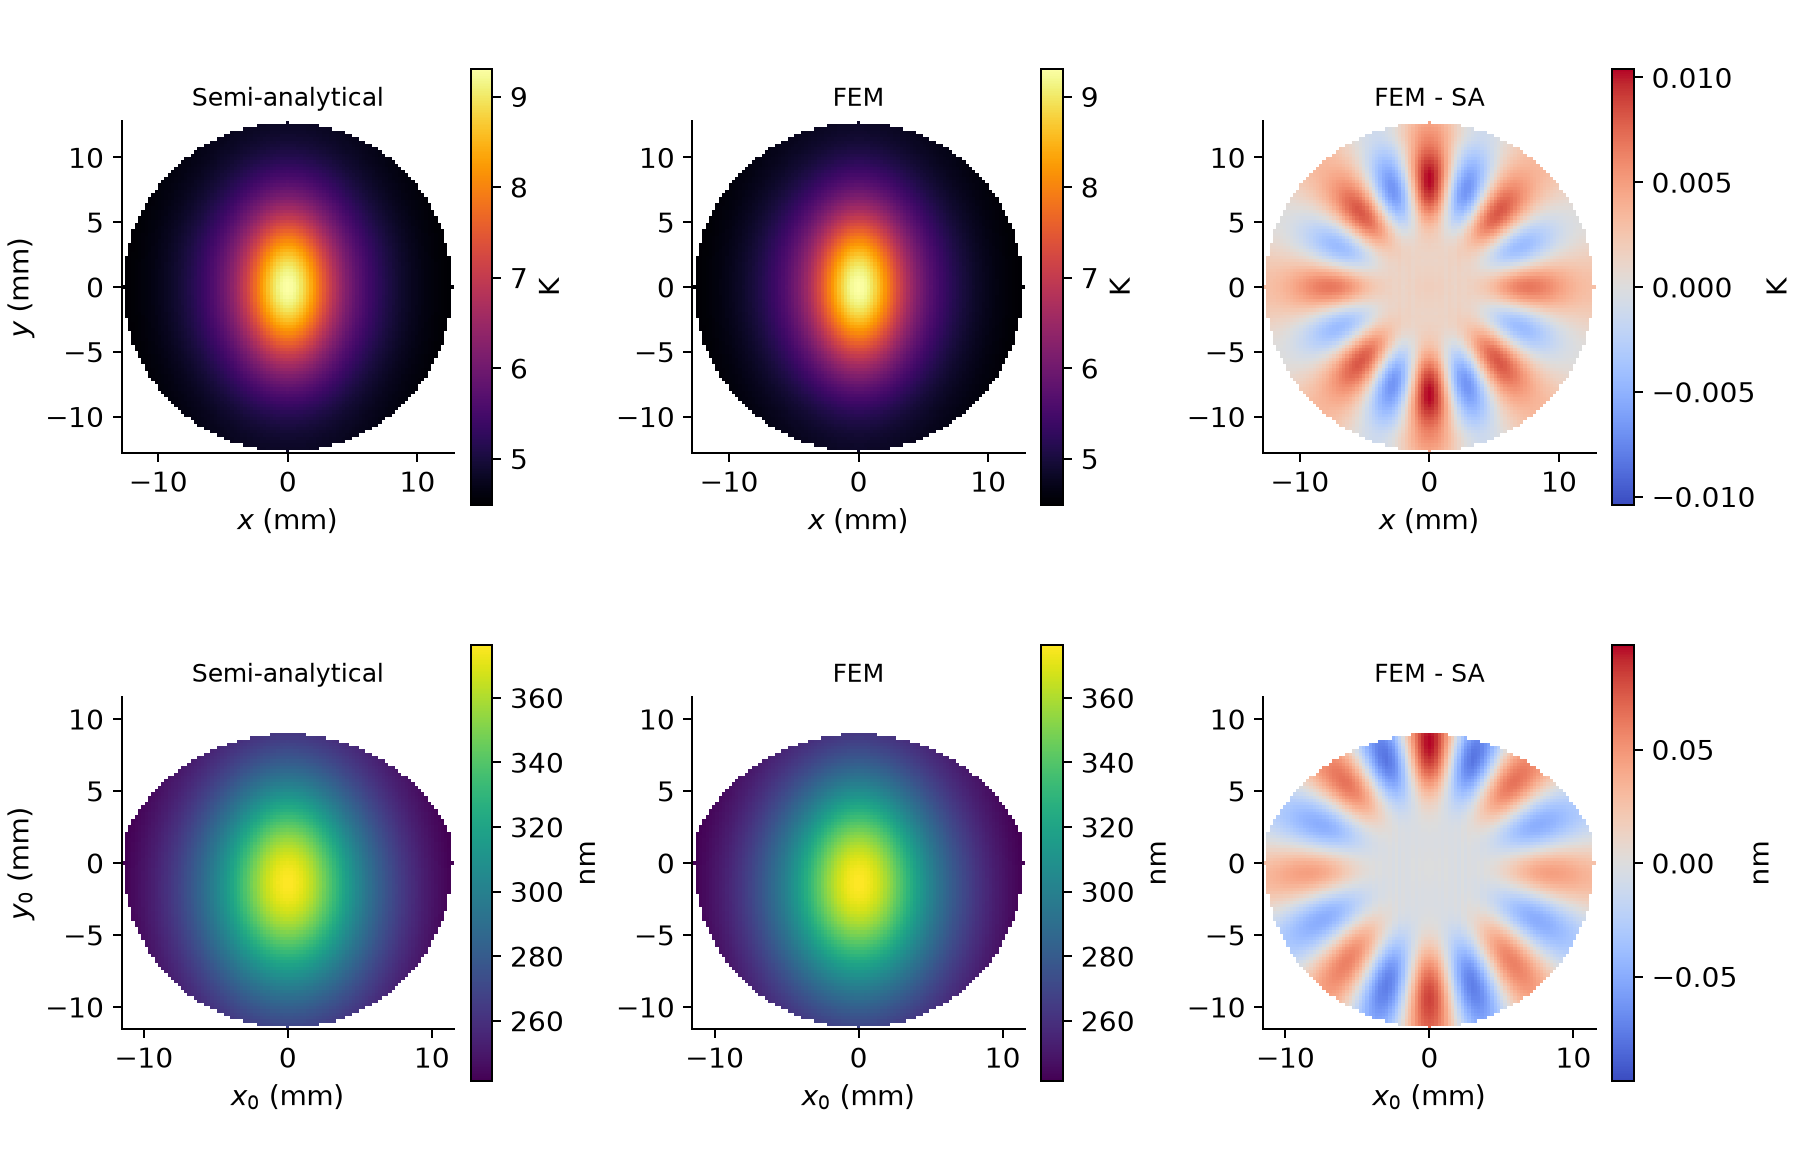
\includegraphics[width=\linewidth]{steady_fem_comparison.png}
\caption{Steady $60^\circ$ distribution comparison on the common domain: semianalytical field, finest finite-element field, and finite-element minus semianalytical difference. Top: front-plane temperature rise. Bottom: refracted-ray OPD, with piston removed from the difference. The two methods use independent thermal representations.}
\label{fig:steadyfem}
\end{figure}
\FloatBarrier
\end{document}
